\section{Auswertung}
\label{sec:auswertung}

In dem Versuch wird die Molwärme $C\ua{p}$ nach Formel \eqref{eq:c_p}
bestimmt. Die in Kapitel \ref{sec:tabellen} enthaltene Tabelle \ref{tab: c_p}
zeigt die Ergebnisse der Wärmekapazität $C\ua{p}$ für verschiedene Temperaturen.

\subsection{Wärmekapazität $C\ua{V}$}

Aus der Wärmekapazität bei konstantem Druck $C\ua{p}$ kann
durch den Zusammenhang \eqref{eqn:c_p-c_v} berechnet werden.
Der Verlauf der aus den Messdaten errechneten Wärmekapazität $C\ua{V}$
für verschiedene Temperaturen $T$ ist in Abb. \ref{fig:c_v} dargestellt.
Für das Kompressionsmodul $\kappa$ wird der Wert $\kappa = \SI{140}{\giga\pascal}$
angenommen~\cite{kompression}.

\begin{figure}
  \centering
  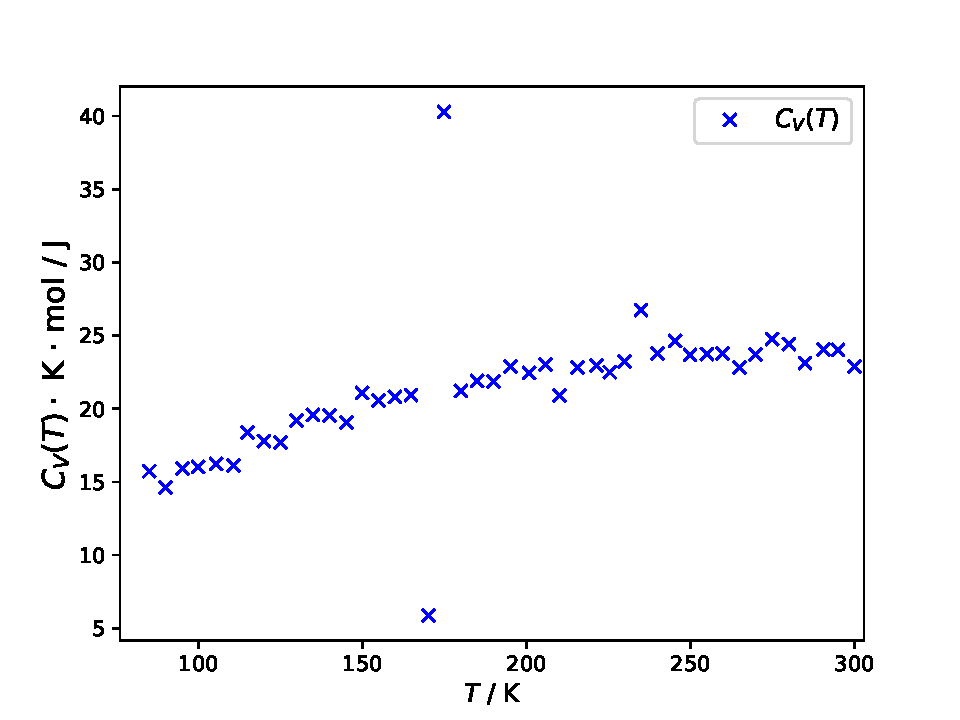
\includegraphics[width = 0.8\textwidth]{Plots/C_V.pdf}
  \caption{Daten der Wärmekapazität für steigende Temperaturen.}
  \label{fig:c_v}
\end{figure}

Es wird ersichtlich, dass in Abb. \ref{fig:c_v} Werte auftauchen, die sehr
stark erwarteten Trend abweichen.
Diese Abweichung wird auf zwei vermutlich fehlerhafte Messdaten in der Zeitmessung zurückgeführt.
Eine Darstellung von $C\ua{V}$ ohne diese beiden Messdaten ist in Abb. \ref{fig:c_v_korrektur}
einzusehen.

\begin{figure}
  \centering
  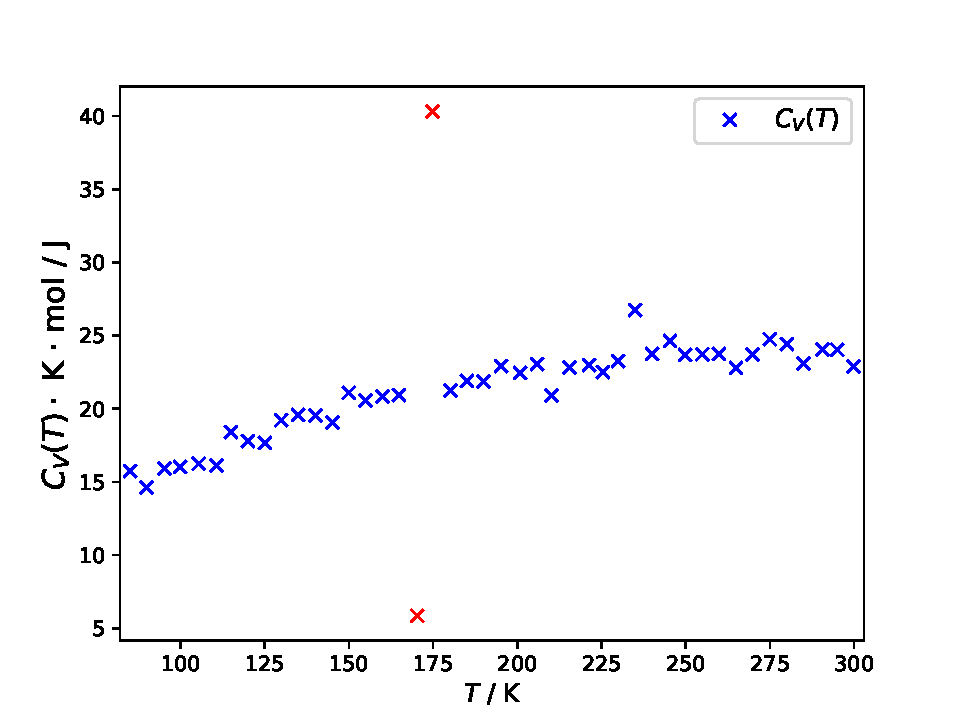
\includegraphics[width = 0.8\textwidth]{Plots/C_V_korrektur.pdf}
  \caption{Angepasste Daten der Wärmekapazität für steigende Temperaturen.}
  \label{fig:c_v_korrektur}
\end{figure}

\subsection{Debye-Funktion}

\subsection{Berechnung von $\omega\ua{D}$ und $\Theta\ua{D}$}

Die Debye-Frequenz $\omega\ua{D}$ wird wie in dem Abschnitt zu Formel \eqref{eqn:omega_D}
beschrieben errechnet.
Für die einzelnen Größen ergeben sich die folgenden Werte.

\begin{align*}
  m\ua{Probe} &= \SI{342}{\gram} \text{~\cite{anleitung}}\\
  M\ua{Cu} &= \SI{63.55}{\dalton}\cdot N\ua{A} \text{~\cite{cu_mass}}\\
  v\ua{l} &= \SI{4.7}{\meter\per\second}\\
  v\ua{t} &= \SI{2.26}{\meter\per\second}\\
  N_L &= \num{3.24e24} \\
  V &= L^3 = V_0\cdot\frac{m}{M}\approx \SI{0.382}{\centi\meter^3}\\
  \omega\ua{D} &\approx \SI{43.5e12}{\per\second}\\
  \Theta\ua{D} &\approx \SI{322.21}{\kelvin}
\end{align*}

\section{Diskussion}
\label{sec:diskussion}

\newpage
\section{Tabellen}
\label{sec:tabellen}
\pagestyle{empty}
\begin{table}[b!]
\vspace{-10pt}
\centering
\caption{Messdaten zu der Wärmekapazität $C\ua{p}$}
\label{tab: c_p}
\begin{tabular}{S S S S S }
\toprule
{$C\ua{p} / \si{\joule \per \kelvin \per \mol}$} & {$U / \si{\volt}$} & {$ I / \si{\milli\ampere}$} & {$ \increment t / \si{\s}$} & {$ \increment T / \si{\kelvin}$}  \\
\midrule
 15.79  & 15.79  & 150.90  & 210  & 5.89\\
14.68  & 15.87  & 151.55  & 163  & 4.96\\
15.99  & 15.85  & 151.25  & 187  & 5.21\\
16.12  & 15.80  & 150.65  & 173  & 4.75\\
16.36  & 15.82  & 150.70  & 202  & 5.47\\
16.27  & 15.86  & 150.90  & 192  & 5.25\\
18.54  & 15.88  & 151.10  & 179  & 4.30\\
17.93  & 15.89  & 151.25  & 202  & 5.03\\
17.85  & 15.88  & 151.00  & 202  & 5.04\\
19.39  & 15.87  & 150.75  & 210  & 4.81\\
19.78  & 15.89  & 150.85  & 225  & 5.07\\
19.77  & 15.91  & 150.95  & 225  & 5.08\\
19.30  & 15.91  & 151.00  & 220  & 5.09\\
21.34  & 15.93  & 151.05  & 232  & 4.86\\
20.83  & 15.89  & 150.70  & 228  & 4.87\\
21.10  & 15.86  & 150.35  & 244  & 5.12\\
21.23  & 15.88  & 150.45  & 234  & 4.89\\
6.18  & 15.88  & 150.50  & 75  & 5.39\\
40.64  & 15.89  & 150.50  & 427  & 4.67\\
21.59  & 15.89  & 150.55  & 251  & 5.17\\
22.28  & 15.91  & 150.60  & 247  & 4.94\\
22.24  & 15.91  & 150.65  & 247  & 4.95\\
23.28  & 15.91  & 150.70  & 272  & 5.20\\
22.85  & 15.91  & 150.70  & 293  & 5.71\\
23.45  & 15.92  & 150.70  & 262  & 4.98\\
21.34  & 15.92  & 150.70  & 203  & 4.24\\
23.27  & 15.92  & 150.75  & 287  & 5.50\\
23.45  & 15.92  & 150.80  & 303  & 5.76\\
22.99  & 15.93  & 150.80  & 207  & 4.02\\
23.74  & 15.93  & 150.80  & 241  & 4.53\\
27.25  & 15.92  & 150.80  & 308  & 5.04\\
24.28  & 15.92  & 150.85  & 275  & 5.05\\
25.18  & 15.92  & 150.90  & 300  & 5.32\\
24.24  & 15.92  & 150.90  & 248  & 4.57\\
24.32  & 15.92  & 150.90  & 277  & 5.08\\
24.35  & 15.92  & 150.90  & 264  & 4.84\\
23.43  & 15.92  & 150.90  & 268  & 5.11\\
24.34  & 15.92  & 150.90  & 265  & 4.86\\
25.42  & 15.91  & 150.90  & 292  & 5.13\\
25.10  & 15.91  & 150.95  & 289  & 5.14\\
23.82  & 15.91  & 151.00  & 261  & 4.89\\
24.78  & 15.91  & 151.00  & 315  & 5.67\\
24.79  & 15.91  & 151.00  & 244  & 4.39\\
23.68  & 15.91  & 151.00  & 261  & 4.92\\
\bottomrule
\end{tabular}
\end{table}

